%%%%%%%%%%%%%%%%%%%%%%%%%%%%%%%%%%%%%%%%%%%%%%%%%%%%%%%%%%%%%%%%%%%%%%%%%%%%%%%
%
% Tommy P. Keane
% Master of Science Thesis
% Department of Electrical and Microelectronic Engineering
%
% March 2011
%
%
%
% .tex and .sty modified from:
% http://www.ce.rit.edu/studentresources/gradresource/LaTexThesis.zip
%
%%%%%%%%%%%%%%%%%%%%%%%%%%%%%%%%%%%%%%%%%%%%%%%%%%%%%%%%%%%%%%%%%%%%%%%%%%%%%%%

%%%%%%%%%%%%%%%%%%%%%%%%%%%%%%%%%%%%%%%%%%%%%%%%%%%%%%%%%%%%%%%%%%%%%%%%%%%%%%%
%
% CHAPTER 5
%
% SECTION 2: Near-Affine Views
%
%%%%%%%%%%%%%%%%%%%%%%%%%%%%%%%%%%%%%%%%%%%%%%%%%%%%%%%%%%%%%%%%%%%%%%%%%%%%%%%


%%%%%%%%%%%%%%%%%%%%%%%%%%%%%%%%%%%%%%%%%%%%%%%%%%%%%%%%%%%%%%%%%%%%%%%%%%%%%%%
% BEGIN DOCUMENT

The affine related views of the previous section are entirely unrealistic, as stated, but in making a slow transition to evaluate the algorithm in realistic scnearios, views with near-affine relations can be generated in reality. In Figure \ref{ArtGallery4Images5} the views are not affine related, but being that there is only a slight rotation between the views (the right view's camera was rotated only a few degrees along the horizontal axis in-line with the camera centers) there is almost no occlusion or parallax disparity, and there is very little depth variation between the views. While all these characteristics (occlusion, parallax, depth) do exist in the views, they are minimal enough that they can be ignored and an affine homography should perform quite well in registering the views.

% ART GALLERY 4 - 005
\begin{figure}[h]
\centering
\subfigure{ 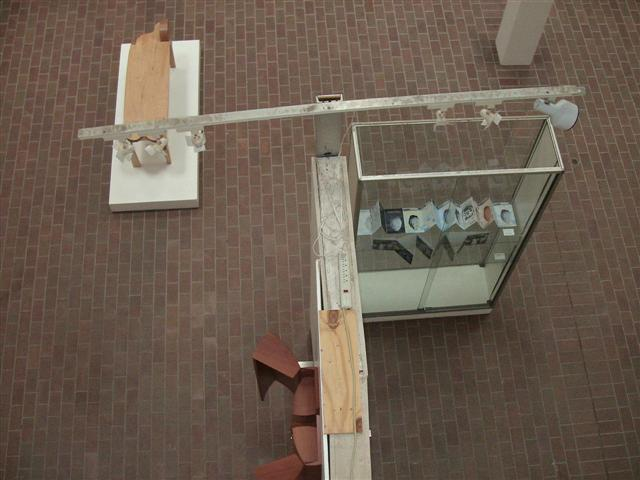
\includegraphics[width=.4\textwidth]{AGS4L005} \label{AGS4L005} }
\subfigure{ 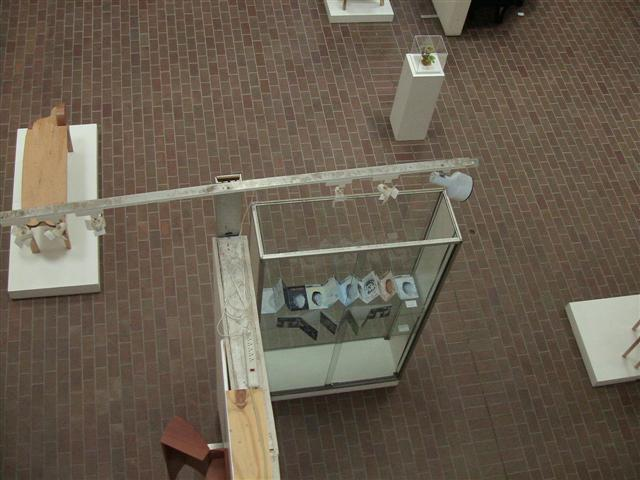
\includegraphics[width=.4\textwidth]{AGS4R005} \label{AGS4R005} }
\caption{Art Gallery Scene (a) Left View, (b) Right View}
\label{ArtGallery4Images5}
\end{figure}

Applying the WFMI algorithm to the views from Figure \ref{ArtGallery4Images5} produces the automatically generated panorama in Figure \ref{ArtGallery4Stitched5} with a manually generated panorama presented in Figure \ref{ArtGallery4StitchedManual5}.

\begin{figure}[h]
\centering
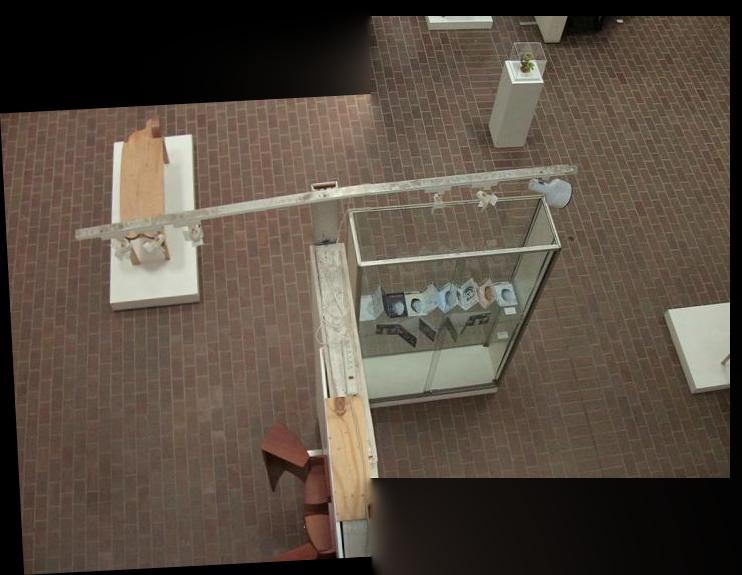
\includegraphics[width=1\textwidth]{AGS4SP005005}
\caption{Art Gallery Views Blended}
\label{ArtGallery4Stitched5}
\end{figure}

\begin{figure}[h]
\centering
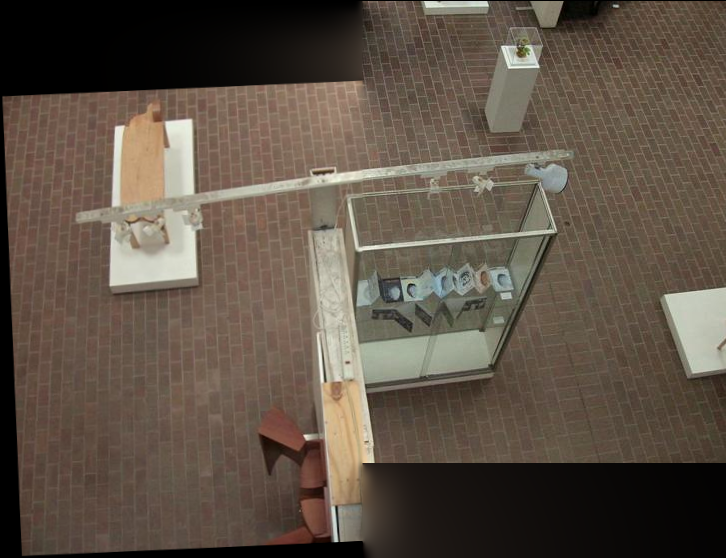
\includegraphics[width=1\textwidth]{AGS4SP005ManAff}
\caption{Art Gallery Views Blended Manually (Affine)}
\label{ArtGallery4StitchedManual5}
\end{figure}


% ART GALLERY 4 - 007
\begin{figure}[h]
\centering
\subfigure{ 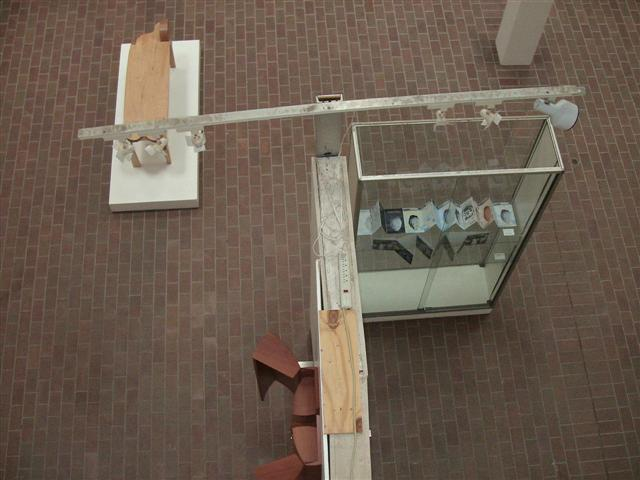
\includegraphics[width=.4\textwidth]{AGS4L007} \label{AGS4L007} }
\subfigure{ 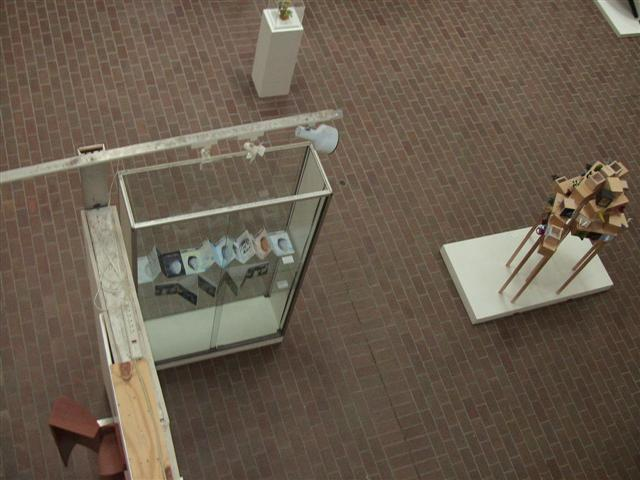
\includegraphics[width=.4\textwidth]{AGS4R007} \label{AGS4R007} }
\caption{Art Gallery Scene (Modest Angle) Views (a) Left View, (b) Right View}
\label{ArtGallery4Images7}
\end{figure}

\begin{figure}[h]
\centering
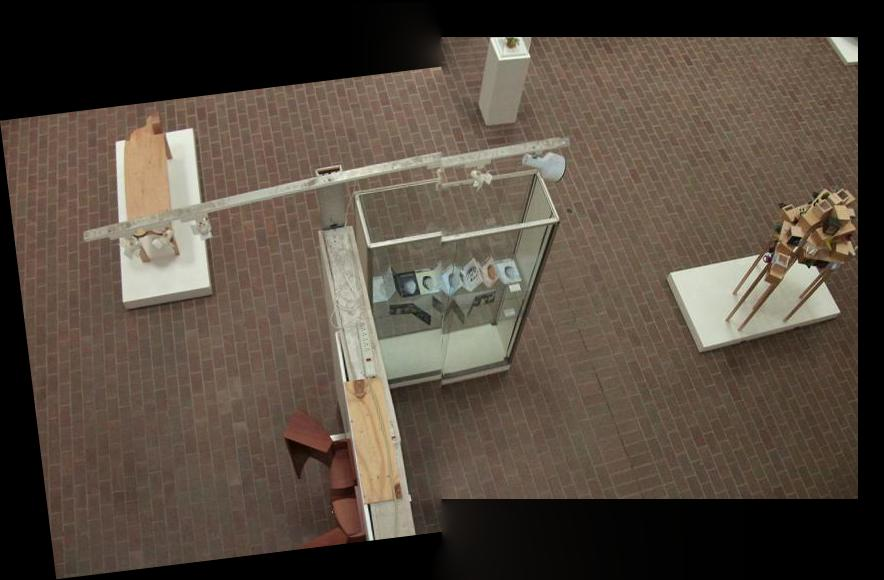
\includegraphics[width=1\textwidth]{AGS4SP007007}
\caption{Art Gallery (Modest Angle) Views Blended}
\label{ArtGallery4Stitched7}
\end{figure}


% ART GALLERY 4 - 008
\begin{figure}[h]
\centering
\subfigure{ 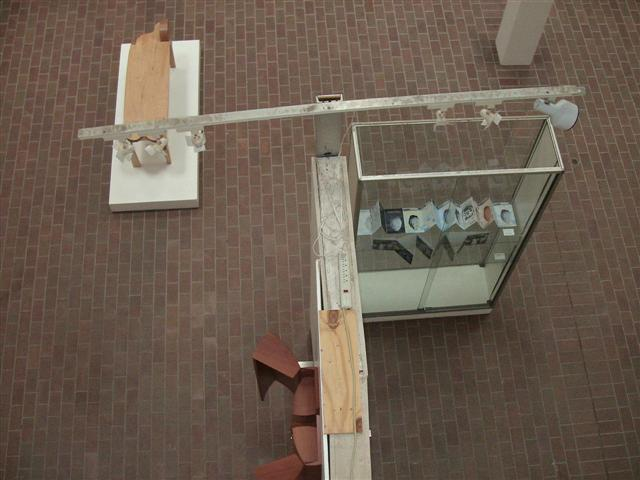
\includegraphics[width=.4\textwidth]{AGS4L008} \label{AGS4L008} }
\subfigure{ 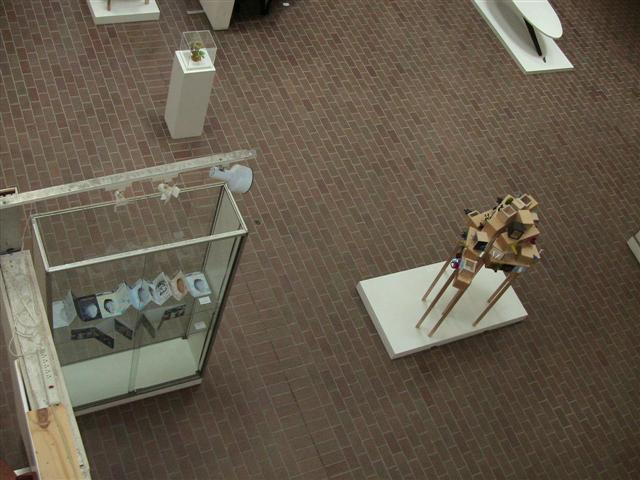
\includegraphics[width=.4\textwidth]{AGS4R008} \label{AGS4R008} }
\caption{Art Gallery (Large Angle) Views (a) Left View, (b) Right View}
\label{ArtGallery4Images8}
\end{figure}

\begin{figure}[h]
\centering
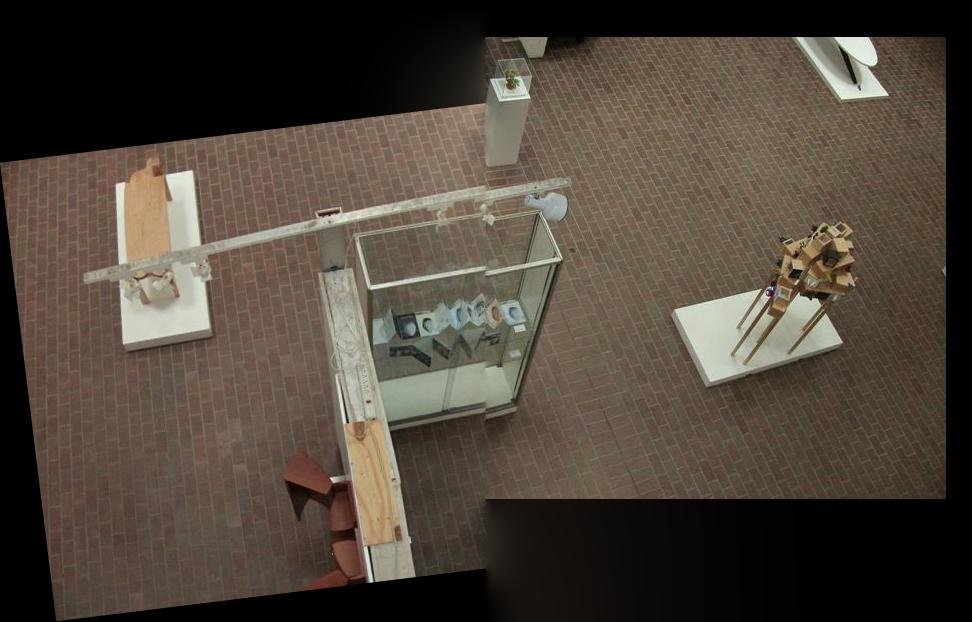
\includegraphics[width=1\textwidth]{AGS4SP008008}
\caption{Art Gallery (Large Angle) Views Blended}
\label{ArtGallery4Stitched8}
\end{figure}



%%%%%%%%%%%%%%%%%%%%%%%%%%%%%%%%%%%%%%%%%%%%%%%%%%%%%%%%%%%%%%%%%%%%%%%%%%%%%%%
% END OF DOCUMENT

